\chapter{An Unconference Software Solution}
\section{UnconfRS}
UnconfRS is a full stack web application that allows users to propose sessions and vote on sessions they are interested in. They can also view a populated schedule that contains information about the session and where the session is located. Additionally there is functionality for admin and facilitators to make edits to sessions others have submitted (e.g. choosing a more appropriate tag for a session). The admin alone can generate a schedule which uses the known information of who is putting on a session at a specific time and which sessions users expressed interest in to attempt to create a best schedule. The admin also has fine control with being able to drag and drop the sessions already on the schedule. 
\subsection{Creating an agenda}
There are three main steps for a user to participate in agenda creation: registering a new account through the UnconfRS website, proposing sessions on the sessions page, and voting on sessions they would like to attend.\\

\subsection{Scheduling For UnconfRS}
Once an agenda has been created, the admin needs to create the schedule. The first step in that process is clicking the button Populate Schedule on the unconf schedule page. This attempts to create a best schedule that avoids conflicts and tries to make sure people are able to see the sessions they want. At this point the admin can make manual changes to the schedule as well. They can remove or add to the schedule, as well as drag and drop sessions on the schedule to move when the sessions are happening.\\

\section{Implementation}
This section describes the technical decisions for the implementation of UnconfRS. From the choice of Rust as the programming language, system design and architecture, frontend, backend, database, security, and the scheduling approach.

\subsection{Why Rust}
Rust was chosen because it is a modern programming language that provides performance, reliability, and productivity. The scheduler needs to evaluate many candidate solutions quickly, so a performant language was desired. The type system and ownership model ensure many potential bugs are caught at compile time. Additionally, the existing ecosystem of crates meets the majority of the needs for this project.
%"https://rust-lang.org/"\\
%Performance, Reliability, Productivity
\subsection{System Design and Architecture}
The makeup of UnconfRS can be divided up into three main parts consisting of a Rust-based backend (Axum), PostgreSQL database (SQLx), and a mostly server-side rendered frontend (Askama) with JavaScript enhancements.\\
\\The project is organized as three Cargo workspaces: \texttt{server}, \texttt{scheduler}, and \texttt{test data creation}. The \texttt{server} workspace contains all aspects relating to the frontend, backend, and database. The \texttt{scheduler} workspace contains the scheduling library that gets used when generating a schedule. The \texttt{test data creation} workspace contains a utility for generating test data. Having the separate workspaces makes it clear what the code in the workspace is responsible for. It also has the benefit of lowering compilation time.\\
\\Overall the web application follows an MVC (Model View Controller) architecture design pattern, where models manage data/business logic, views handle the user interface, and controllers act as an intermediary between models and views. This pattern provides a straightforward way for separating code according to specific responsibilities.
\begin{figure}[h]
    \centering
    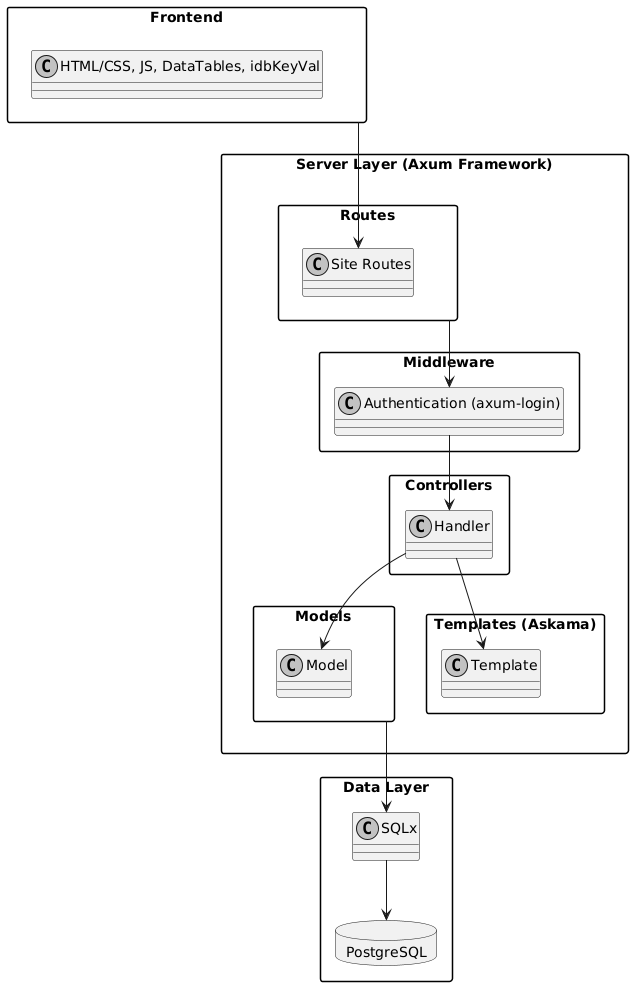
\includegraphics[width=0.85\linewidth]{figs/high_level_diagram.png}
    \caption{High level diagram showing the different areas of implementation}
    \label{fig:enter-label}
\end{figure}
\clearpage
\subsection{Frontend}
The frontend utilizes Askama for server-side template rendering, chosen for its compile time type safety. DataTables is used for displaying the table of sessions in a responsive and interactive manner. Bootstrap 5.3.8 is utilized for responsive styling. The HTML 5 Drag and Drop API is used to allow for schedule manipulation. For client-side storage, IDB-Keyval is used.

\subsection{Backend}
The backend is built with Axum (by Tokio), which is a web application framework written in Rust that focuses on ergonomics and modularity. It uses the Tokio async runtime for concurrent I/O. Axum was chosen here due to prior familiarity and its growing adoption in the Rust community. For middleware and authentication/authorization various Tower crates and axum-login are used. For serializing and deserializing data structures Serde is used.

\subsection{Database}
For the database, PostgreSQL was chosen mostly due to prior familiarity, but it is also a powerful open source relational database system. For working with the database in the backend, the crate SQLx was chosen. This was chosen due to it featuring compile time checked queries.

\subsection{Security Considerations}
UnconfRS implements session-based authentication and role-based authorization for access to the application.\\\\
\textbf{Authentication}:
The application uses axum-login for session-based authentication. The passwords are stored hashed using bcrypt.\\
Login workflow:
\begin{enumerate}
    \item User submits Unconference password in order to access the site
    \item On success a server-side session is created in PostgreSQL
    \item Session ID is stored in a secure HTTP only cookie
    \item User submits credentials in the account login form
    \item On success a new session associated to the logged in user replaces the one for site access (in the database and in the cookie)
\end{enumerate}

\textbf{Authorization}:
Permission based access is implemented also using axum-login with different levels of access:

\begin{table}[hbtp]
    \centering
    \begin{tabular}{|m{12em}| ccccc|}
      \hline
     ~ & \multicolumn{2}{|c}{Unauthorized} & \multicolumn{3}{c|}{Authorized} \\
     \hline
     Scenarios & Public & User & User & Staff & Admin\\
     \hline
         Unconf login page &  \checkmark & \checkmark & \checkmark & \checkmark & \checkmark\\
         \hline
         Read-only site access & X & \checkmark & \checkmark & \checkmark & \checkmark\\
         \hline
         CRUD actions on their own sessions & X & X & \checkmark & \checkmark & \checkmark\\
         \hline
         Voting on sessions & X & X & \checkmark & \checkmark & \checkmark\\
         \hline
         CRUD actions on any sessions & X & X & X & \checkmark & \checkmark\\
         \hline
         Create session for a user & X & X & X & \checkmark & \checkmark\\
         \hline
         Register user on their behalf & X & X & X & \checkmark & \checkmark\\
         \hline
         CRUD actions for tags & X & X & X & X & \checkmark \\
         \hline
         Schedule setup (adding rooms and timeslots) & X & X & X & X & \checkmark \\
         \hline
         Manipulating the schedule (adding/removing sessions to the schedule or running the scheduler) & X & X & X & X & \checkmark \\
         \hline
    \end{tabular}
    \caption{Actions unauthorized/authorized users can take depending on their role}
    \label{tab:placeholder}
\end{table}
\FloatBarrier
%\begin{itemize}
%    \item \textbf{User} (default): Can submit sessions, update/delete sessions %they created, vote for sessions, and view the schedule
%    \item \textbf{Facilitator} (staff): Can do all that a User can, but they can %also create sessions on behalf of a user, make edits to any session, and register %a user on their behalf, 
%    \item \textbf{Admin} (superuser): Can do all that Staff can, but they can %also create/update/delete the tags that sessions can use, perform the setup for %the schedule (adding rooms and timeslots), and manipulation of the schedule %(adding sessions manually or running the scheduler).
%\end{itemize}

%How the application utilizes authorization and authentication:
%\begin{itemize}
%    \item \textbf{Routes}: Routes are broken up into 5 parts:
%    \begin{itemize}
%        \item No Unconference authentication (can only access Unconference login)
%        \item Unconference authentication but no account authentication (read %only view with User level permissions)
%        \item Unconference authentication and account authentication at User %permission level (read/write access with User level permissions)
%        \item Unconference authentication and account authentication at %Facilitator permission level (read/write access with Facilitator level %permissions)
%        \item Unconference authentication and account authentication at Admin %permission level (read/write access with Admin level permissions)
%    \end{itemize}
%    \item \textbf{Middleware}: Routes utilize middleware to ensure users have the %specified permissions
%    \item \textbf{Ownership}: The application makes sure sessions can only be %updated by the users that created them or by Admin/Facilitators
%    \item \textbf{Askama Templating}: By passing the Askama templates the %permission levels we can conditionally include source files that require higher %level of permissions
%\end{itemize}
\subsection{Scheduling}
As mentioned in the previous scheduling chapter, trying to create schedules for Unconferences creates a state space that would take an unreasonable amount of time to search. The application has access to data so instead of an uninformed brute force search an informed search can be done. The scheduler has access to the number of votes each session received, session tag ID, session speaker ID, and which sessions each speaker voted for. Having that information, heuristics can be created to apply a score to the schedule, where the score is a collection of penalties assessed based on the data. Then we can use local search for the strategy on trying to find the best schedule.

\subsubsection{Heuristics}
For the scheduler the heuristics are made up of five penalty functions that assess scores based on scenarios that lead to a worse schedule. \\\\
%
%
\textbf{Penalize Conflicting Popular Sessions}: For each timeslot, it sorts the sessions, then sums the products of adjacent pairs by their vote counts. This ends up with higher scores for schedules that have high vote sessions happening at the same time as other high vote sessions.
\begin{pseudocode}{Penalty for concurrent popular sessions}
    %\begin{tabbing}Penalty {\bf for} multiple concurrent popular sessions across $Timeslots$$:$\\
%$~~~~$$popular\_conflict$ $\leftarrow$ $0$\\
%$~~~~${\bf for} $i$ {\bf in} $0..$length($Timeslots$)$-1$\\
%$~~~~~~~~$$sorted$ $\leftarrow$ sort $Timeslots$$[$$i$$]$ by votes descending\\
%$~~~~~~~~$$popular\_conflict\_slot$ $\leftarrow$ $0$\\
%$~~~~~~~~${\bf for} $j$ {\bf in} $0..$length($sorted$)$-2$\\
%$~~~~~~~~~~~~$$popular\_conflict\_slot$ $\leftarrow$ $popular\_conflict\_slot$ $+$ $sorted$$[$$j$$]$ %$*$ $sorted$$[$$j$ $+$ $1]$\\
%$~~~~~~~~$$popular\_conflict$ $\leftarrow$ $popular\_conflict$ $+$ $popular\_conflict\_slot$\\
%$~~~~${\bf return} $popular\_conflict$\\
%\end{tabbing}
\begin{tabbing}Penalty {\bf for} multiple concurrent popular sessions across $\textit{Timeslots}$$:$\\
$~~~~$$\textit{popular\_conflict}$ $\leftarrow$ $0$\\
$~~~~${\bf for} $\textit{i}$ {\bf in} $0..$length($\textit{Timeslots}$)$-1$\\
$~~~~~~~~$$\textit{sorted}$ $\leftarrow$ sort $\textit{Timeslots}$$[$$\textit{i}$$]$ by votes descending\\
$~~~~~~~~$$\textit{popular\_conflict\_slot}$ $\leftarrow$ $0$\\
$~~~~~~~~${\bf for} $\textit{j}$ {\bf in} $0..$length($\textit{sorted}$)$-2$\\
$~~~~~~~~~~~~$$\textit{popular\_conflict\_slot}$ $\leftarrow$ $\textit{popular\_conflict\_slot}$ $+$ $\textit{sorted}$$[$$\textit{j}$$]$ $*$ $\textit{sorted}$$[$$\textit{j}$ $+$ $1]$\\
$~~~~~~~~$$\textit{popular\_conflict}$ $\leftarrow$ $\textit{popular\_conflict}$ $+$ $\textit{popular\_conflict\_slot}$\\
$~~~~${\bf return} $\textit{popular\_conflict}$\\
\end{tabbing}
\end{pseudocode}

\textbf{Penalize Popular Session Missing}: This penalty function goes through every scheduled session and compares it with every unscheduled session. For every unscheduled session that has more votes than the scheduled one, a penalty is added proportional to the difference of votes.
\begin{pseudocode}{Penalty for popular sessions missing from the schedule}
    % \begin{tabbing}Penalty {\bf for} sessions {\bf in} $Unassigned\_Sessions$ list more popular than {\bf in} $Assigned\_Sessions$ list$:$\\
% $~~~~$$missing\_popular\_sessions$ $\leftarrow$ $0$\\
% $~~~~${\bf for} each $Assigned$ session {\bf in} $Assigned\_Sessions$$:$\\
% $~~~~~~~~$$missing\_popular\_sessions\_slot$ $\leftarrow$ $0$\\
% $~~~~~~~~${\bf for} each $Unassigned$ session {\bf in} $Unassigned\_Sessions$$:$\\
% $~~~~~~~~~~~~${\bf if} $Unassigned$ $>$ $Assigned$\\
% $~~~~~~~~~~~~~~~~$$difference$ $\leftarrow$ $Unassigned$ $-$ $Assigned$\\
% $~~~~~~~~~~~~~~~~$$missing\_popular\_sessions\_slot$ $\leftarrow$ $missing\_popular\_sessions\_slot$ $+$ $difference$\\
% $~~~~~~~~$$missing\_popular\_sessions\_slot$ $\leftarrow$ $missing\_popular\_sessions\_slot$ $*$ $15$\\
% $~~~~~~~~$$missing\_popular\_sessions$ $\leftarrow$ $missing\_popular\_sessions$ $+$ $missing\_popular\_sessions\_slot$\\
% $~~~~${\bf return} $missing\_popular\_sessions$\\
% \end{tabbing}
\begin{tabbing}Penalty {\bf for} sessions {\bf in} $\textit{Unassigned\_Sessions}$ list more popular than {\bf in} $\textit{Assigned\_Sessions}$ list$:$\\
$~~~~$$\textit{missing\_popular\_sessions}$ $\leftarrow$ $0$\\
$~~~~${\bf for} each $\textit{Assigned}$ session {\bf in} $\textit{Assigned\_Sessions}$$:$\\
$~~~~~~~~$$\textit{missing\_popular\_sessions\_slot}$ $\leftarrow$ $0$\\
$~~~~~~~~${\bf for} each $\textit{Unassigned}$ session {\bf in} $\textit{Unassigned\_Sessions}$$:$\\
$~~~~~~~~~~~~${\bf if} $\textit{Unassigned}$ $>$ $\textit{Assigned}$\\
$~~~~~~~~~~~~~~~~$$\textit{difference}$ $\leftarrow$ $\textit{Unassigned}$ $-$ $\textit{Assigned}$\\
$~~~~~~~~~~~~~~~~$$\textit{missing\_popular\_sessions\_slot}$ $\leftarrow$ $\textit{missing\_popular\_sessions\_slot}$ $+$ $\textit{difference}$\\
$~~~~~~~~$$\textit{missing\_popular\_sessions\_slot}$ $\leftarrow$ $\textit{missing\_popular\_sessions\_slot}$ $*$ $15$\\
$~~~~~~~~$$\textit{missing\_popular\_sessions}$ $\leftarrow$ $\textit{missing\_popular\_sessions}$ $+$ $\textit{missing\_popular\_sessions\_slot}$\\
$~~~~${\bf return} $\textit{missing\_popular\_sessions}$\\
\end{tabbing}
\end{pseudocode}

\textbf{Penalize Late Popular Sessions}: For each timeslot, it sorts the sessions, then sums the products of adjacent pairs by their vote counts. Each timeslot sum is multiplied by timeslot index before being added to the total sum. This ends up with popular sessions that happen later in the day incurring a larger penalty.
\begin{pseudocode}{Penalty for popular sessions occurring later in the day.}
    % \begin{tabbing}Penalty {\bf for} late popular sessions {\bf in} $Timeslots$$:$\\
% $~~~~$$late\_popular\_sessions$ $\leftarrow$ $0$\\
% $~~~~${\bf for} $i$ {\bf in} $0..$length($Timeslots$)$-1$\\
% $~~~~~~~~$$sorted$ $\leftarrow$ sort $Timeslots$$[$$i$$]$ by votes descending\\
% $~~~~~~~~$$late\_popular\_sessions\_slot$ $\leftarrow$ $0$\\
% $~~~~~~~~${\bf for} $j$ {\bf in} $0..$length($sorted$)$-2$\\
% $~~~~~~~~~~~~$$late\_popular\_sessions\_slot$ $\leftarrow$ $late\_popular\_sessions\_slot$ $+$ $sorted$$[$$j$$]$ $*$ $sorted$$[$$j$ $+$ $1]$\\
% $~~~~~~~~$$late\_popular\_sessions$ $\leftarrow$ $late\_popular\_sessions$ $+$ $late\_popular\_sessions\_slot$ $*$ $i$\\
% $~~~~${\bf return} $late\_popular\_sessions$\\
% \end{tabbing}
\begin{tabbing}Penalty {\bf for} late popular sessions {\bf in} $\textit{Timeslots}$$:$\\
$~~~~$$\textit{late\_popular\_sessions}$ $\leftarrow$ $0$\\
$~~~~${\bf for} $\textit{i}$ {\bf in} $0..$length($\textit{Timeslots}$)$-1$\\
$~~~~~~~~$$\textit{sorted}$ $\leftarrow$ sort $\textit{Timeslots}$$[$$\textit{i}$$]$ by votes descending\\
$~~~~~~~~$$\textit{late\_popular\_sessions\_slot}$ $\leftarrow$ $0$\\
$~~~~~~~~${\bf for} $\textit{j}$ {\bf in} $0..$length($\textit{sorted}$)$-2$\\
$~~~~~~~~~~~~$$\textit{late\_popular\_sessions\_slot}$ $\leftarrow$ $\textit{late\_popular\_sessions\_slot}$ $+$ $\textit{sorted}$$[$$\textit{j}$$]$ $*$ $\textit{sorted}$$[$$\textit{j}$ $+$ $1]$\\
$~~~~~~~~$$\textit{late\_popular\_sessions}$ $\leftarrow$ $\textit{late\_popular\_sessions}$ $+$ $\textit{late\_popular\_sessions\_slot}$ $*$ $\textit{i}$\\
$~~~~${\bf return} $\textit{late\_popular\_sessions}$\\
\end{tabbing}
\end{pseudocode}

\textbf{Penalize Same Topic Timeslots}: This penalty function iterates each of the timeslots. Within each timeslot, construct a HashMap that tracks for each tag\_id the total votes and number of occurrences. For every item in the HashMap add to the penalty score equal to $votes$ $*$ $($$count$ $-$ $1$$)$.
\begin{pseudocode}{Penalty for multiple sessions in the same timeslot having the same topic.}
    % \begin{tabbing}Penalty {\bf for} concurrent $sessions$ with same $tag\_id$ {\bf in} $Timeslots$$:$\\
% $~~~~$$tag\_counts$ $\leftarrow$ initialize empty HashMap of $tag\_id$ $\rightarrow$ ($votes$$,$ $count$)\\
% $~~~~$$tag\_conflict$ $\leftarrow$ $0$\\
% $~~~~${\bf for} $timeslot$ {\bf in} $Timeslots$\\
% $~~~~~~~~$$tag\_counts$ $\leftarrow$ reset the HashMap each iteration\\
% $~~~~~~~~$\\
% $~~~~~~~~${\bf for} $session$ {\bf in} $timeslot$\\
% $~~~~~~~~~~~~${\bf if} $session$$.$$session\_id$ and $session$$.$$tag\_id$ exist\\
% $~~~~~~~~~~~~~~~~$$tag\_counts$$[$$session$$.$$tag\_id$$].$$votes$ $\leftarrow$ $tag\_counts$$[$$session$$.$$tag\_id$$].$$votes$ $+$ $session$$.$$num\_votes$\\
% $~~~~~~~~~~~~~~~~$$tag\_counts$$[$$session$$.$$tag\_id$$].$$count$ $\leftarrow$ $tag\_counts$$[$$session$$.$$tag\_id$$].$$count$ $+$ $1$\\
% \\
% $~~~~~~~~${\bf for} ($votes$$,$ $count$) {\bf in} $tag\_counts$ values\\
% $~~~~~~~~~~~~$$tag\_conflict$ $\leftarrow$ $tag\_conflict$ $+$ $votes$ $*$ ($count$ $-$ $1$)\\
% $~~~~${\bf return} $tag\_conflict$\\
% \end{tabbing}
\begin{tabbing}Penalty {\bf for} concurrent sessions with same $\textit{tag\_id}$ {\bf in} $\textit{Timeslots}$$:$\\
$~~~~$$\textit{tag\_counts}$ $\leftarrow$ initialize empty HashMap of $\textit{tag\_id}$ $\rightarrow$ ($\textit{votes}$$,$ $\textit{count}$)\\
$~~~~$$\textit{tag\_conflict}$ $\leftarrow$ $0$\\
$~~~~${\bf for} $\textit{timeslot}$ {\bf in} $\textit{Timeslots}$\\
$~~~~~~~~$$\textit{tag\_counts}$ $\leftarrow$ reset the HashMap each iteration\\
\\
$~~~~~~~~${\bf for} $\textit{session}$ {\bf in} $\textit{timeslot}$\\
$~~~~~~~~~~~~${\bf if} $\textit{session}$$.$$\textit{session\_id}$ and $\textit{session}$$.$$\textit{tag\_id}$ exist\\
$~~~~~~~~~~~~~~~~$$\textit{tag\_counts}$$[$$\textit{session}$$.$$\textit{tag\_id}$$].$$\textit{votes}$ $\leftarrow$ $\textit{tag\_counts}$$[$$\textit{session}$$.$$\textit{tag\_id}$$].$$\textit{votes}$ $+$ $\textit{session}$$.$$\textit{num\_votes}$\\
$~~~~~~~~~~~~~~~~$$\textit{tag\_counts}$$[$$\textit{session}$$.$$\textit{tag\_id}$$].$$\textit{count}$ $\leftarrow$ $\textit{tag\_counts}$$[$$\textit{session}$$.$$\textit{tag\_id}$$].$$\textit{count}$ $+$ $1$\\
\\
$~~~~~~~~~~~~${\bf for} ($\textit{votes}$$,$ $\textit{count}$) {\bf in} $\textit{tag\_counts}$ values\\
$~~~~~~~~~~~~~~~~$$\textit{tag\_conflict}$ $\leftarrow$ $\textit{tag\_conflict}$ $+$ $\textit{votes}$ $*$ ($\textit{count}$ $-$ $1$)\\
$~~~~${\bf return} $\textit{tag\_conflict}$\\
\end{tabbing}
\end{pseudocode}

\textbf{Penalize Speaker Voting Conflicts}: This penalty function iterates each of the timeslots. For each session, check whether the session's speaker has voted on sessions happening at the same time. For each session happening at the same time that received a vote add to the penalty score the product of the two session vote amounts.
\begin{pseudocode}{Penalty for sessions a speaker has voted for occurring while they are scheduled for leading a session.}
    % \begin{tabbing}Penalty {\bf for} concurrent $sessions$ that conflict with $sessions$ the speaker voted {\bf for} {\bf in} $Timeslots$$:$\\
% $~~~~$$speaker\_conflict$ $\leftarrow$ $0$\\
% $~~~~${\bf for} $i$ {\bf in} $0..$length($Timeslots$) $-$ $1$\\
% $~~~~~~~~$$sessions$ $\leftarrow$ list of $sessions$ at $Timeslots$$[$$i$$]$\\
% $~~~~~~~~$$num\_sessions$ $\leftarrow$ length($sessions$)\\
% $~~~~~~~~$$speaker\_conflict\_slot$ $\leftarrow$ $0$\\
% $~~~~~~~~${\bf for} $j$ {\bf in} $0..$$num\_sessions$ $-$ $1$\\
% $~~~~~~~~~~~~$$speaker\_votes$ $\leftarrow$ the list of $sessions$$[$$j$$].$$speaker\_votes$\\
% $~~~~~~~~~~~~${\bf for} $k$ {\bf in} $0..$$num\_sessions$ $-$ $1$\\
% $~~~~~~~~~~~~~~~~${\bf if} $k$ $!=$ $j$\\
% $~~~~~~~~~~~~~~~~~~~~${\bf if} $sessions$$[$$j$$].$$session\_id$ {\bf in} $speaker\_votes$\\
% $~~~~~~~~~~~~~~~~~~~~~~~~$$session\_j\_votes$ $\leftarrow$ max($sessions$$[$$j$$].$votes$,$ $1$)\\
% $~~~~~~~~~~~~~~~~~~~~~~~~$$session\_k\_votes$ $\leftarrow$ max($sessions$$[$$k$$].$votes$,$ $1$)\\
% $~~~~~~~~~~~~~~~~~~~~~~~~$$speaker\_conflict\_session$ $\leftarrow$ $session\_j\_votes$ $*$ $session\_k\_votes$\\
% $~~~~~~~~~~~~~~~~~~~~~~~~$$speaker\_conflict\_slot$ $\leftarrow$ $speaker\_conflict\_slot$ $+$ $speaker\_conflict\_session$\\
% $~~~~~~~~$$speaker\_conflict$ $\leftarrow$ $speaker\_conflict$ $+$ $speaker\_conflict\_slot$\\
% $~~~~${\bf return} $speaker\_conflict$\\
% \end{tabbing}
\begin{tabbing}Penalty {\bf for} concurrent $\textit{sessions}$ that conflict with $\textit{sessions}$ the speaker voted {\bf for} {\bf in} $\textit{Timeslots}$$:$\\
$~~~~$$\textit{speaker\_conflict}$ $\leftarrow$ $0$\\
$~~~~${\bf for} $\textit{i}$ {\bf in} $0..$$\textit{length}$($\textit{Timeslots}$) $-$ $1$\\
$~~~~~~~~$$\textit{sessions}$ $\leftarrow$ list of $\textit{sessions}$ at $\textit{Timeslots}$$[$$\textit{i}$$]$\\
$~~~~~~~~$$\textit{num\_sessions}$ $\leftarrow$ $\textit{length}$($\textit{sessions}$)\\
$~~~~~~~~$$\textit{speaker\_conflict\_slot}$ $\leftarrow$ $0$\\
$~~~~~~~~${\bf for} $\textit{j}$ {\bf in} $0..$$\textit{num\_sessions}$ $-$ $1$\\
$~~~~~~~~~~~~$$\textit{speaker\_votes}$ $\leftarrow$ the list of $\textit{sessions}$$[$$\textit{j}$$].$$\textit{speaker\_votes}$\\
$~~~~~~~~~~~~${\bf for} $\textit{k}$ {\bf in} $0..$$\textit{num\_sessions}$ $-$ $1$\\
$~~~~~~~~~~~~~~~~${\bf if} $\textit{k}$ $!=$ $\textit{j}$\\
$~~~~~~~~~~~~~~~~~~~~${\bf if} $\textit{sessions}$$[$$\textit{j}$$].$$\textit{session\_id}$ {\bf in} $\textit{speaker\_votes}$\\
$~~~~~~~~~~~~~~~~~~~~~~~~$$\textit{session\_j\_votes}$ $\leftarrow$ max($\textit{sessions}$$[$$\textit{j}$$].$votes$,$ $1$)\\
$~~~~~~~~~~~~~~~~~~~~~~~~$$\textit{session\_k\_votes}$ $\leftarrow$ max($\textit{sessions}$$[$$\textit{k}$$].$votes$,$ $1$)\\
$~~~~~~~~~~~~~~~~~~~~~~~~$$\textit{speaker\_conflict\_session}$ $\leftarrow$ $\textit{session\_j\_votes}$ $*$ $\textit{session\_k\_votes}$\\
$~~~~~~~~~~~~~~~~~~~~~~~~$$\textit{speaker\_conflict\_slot}$ $\leftarrow$ $\textit{speaker\_conflict\_slot}$ $+$ $\textit{speaker\_conflict\_session}$\\
$~~~~~~~~$$\textit{speaker\_conflict}$ $\leftarrow$ $\textit{speaker\_conflict}$ $+$ $\textit{speaker\_conflict\_slot}$\\
$~~~~${\bf return} $\textit{speaker\_conflict}$\\
\end{tabbing}
\end{pseudocode}

\textbf{Weight the Scores}: This function takes the values from the penalty functions (h1, h2, h3, h4, h5) and applies a predetermined modifier to the values based on how important that heuristic is. Then it adds up all the modified values returning a unified score. These weights were determined by trial and error.
\begin{pseudocode}{Weighting the penalty scores}
    \begin{tabbing}Given heuristic values $h1$$,$ $h2$$,$ $h3$$,$ $h4$$,$ and $h5$ {\bf return} a unified score$:$\\
$~~~~$$conflicting$ $\leftarrow$ $0.5$\\
$~~~~$$missing$ $\leftarrow$ $0.75$\\
$~~~~$$late$ $\leftarrow$ $0.1$\\
$~~~~$$same\_tag$ $\leftarrow$ $0.3$\\
$~~~~$$speaker\_conflict$ $\leftarrow$ $0.1$\\
\\
$~~~~${\bf return} $conflicting$ $*$ $h1$ $+$\\
$~~~~~~~~$$missing$ $*$ $h2$ $+$\\
$~~~~~~~~$$late$ $*$ $h3$ $+$\\
$~~~~~~~~$$same\_tag$ $*$ $h4$ $+$\\
$~~~~~~~~$$speaker\_conflict$ $*$ $h5$\\
\end{tabbing}
\end{pseudocode}

\subsubsection{Local Search}
The implementation of local search for this project uses a handful of strategies to try and find an optimal schedule. These strategies are random restarts, minimizing the penalty score, and a simplified simulated annealing.

\textbf{Random Restarts}\\In this strategy the scheduler runs a variable number of times. Each time the scheduler is run a different initial random state for the schedule is created. Only the best of the scheduler runs is kept. The goal of doing this is that by having many different starting states, a global minimum is more likely to be found.
\begin{pseudocode}{Run the scheduler from various random states}
\begin{tabbing}Improve $\textit{schedule}$ with specified number of $\textit{restarts}$$:$\\
$~~~~$$\textit{original\_schedule}$ $\leftarrow$ $\textit{copy}$($\textit{schedule}$)\\
$~~~~$$best\_score$ $\leftarrow$ $schedule$$.$$\textit{improve}$()\\
$~~~~$$best\_data$ $\leftarrow$ $copy$($schedule$)\\
\\
$~~~~${\bf for} $i$ {\bf in} $0..$$restarts$\\
$~~~~~~~~$$schedule$ $\leftarrow$ $copy$($original\_schedule$)\\
$~~~~~~~~$$new\_score$ $\leftarrow$ $schedule$$.$$improve$()\\
$~~~~~~~~${\bf if} $new\_score$ $<$ $best\_score$\\
$~~~~~~~~~~~~$$best\_score$ $\leftarrow$ $new\_score$\\
$~~~~~~~~~~~~$$best\_data$ $\leftarrow$ $copy$($schedule$)\\
\\
$~~~~$$schedule$ $\leftarrow$ $best\_data$\\
$~~~~${\bf return} $best\_score$\\
\end{tabbing}
\end{pseudocode}

\textbf{Coin Flip}\\
Perform a \(\frac{50}{50}\) "coin flip", heads (true), improve the schedule  by minimizing the penalty score this iteration. On tails (false), perform simplified simulated annealing.
\begin{pseudocode}{Find minimum neighbor or perform simulated annealing}
\begin{tabbing}Coinflip$:$\\
$~~~~$$\textit{coin\_flip}$ $\leftarrow$ \(\frac{50}{50}\) random boolean\\
$~~~~${\bf if} $\textit{coin\_flip}$\\
$~~~~~~~~$Minimize the penalty score\\
$~~~~${\bf else}\\
$~~~~~~~~$Perform the simplified simulated annealing\\
\end{tabbing}
\end{pseudocode}

\textbf{Simplified Simulated Annealing}\\
Take a random swappable session and swap it with a different swappable session or an unassigned session. If this improved the schedule, accept the move. Otherwise accept the move with probability \(\frac{search\_iter}{max\_iterations}\). By accepting moves that make the schedule worse early on and fewer as you get closer to the end, you create a more broadly searched space where improvement has a good chance of finding a global minimum.\\\\

\textbf{Minimizing the Penalty Score}\\
For every swappable session on the schedule, try swapping it with swappable sessions after it and all unassigned sessions. Out of all the swaps, if the swap that has the lowest score has a score lower than the original score, then that swap is accepted. The score is updated to reflect that. The goal by taking the best move that can be made is that every step is one towards the best schedule. However, this could lead to a local minimum.
\begin{pseudocode}{Improve the schedule alternating between a best move local search and simulated annealing.}
% \begin{tabbing}Improve $schedule$$:$\\
% $~~~~$$schedule$ $\leftarrow$ randomly fill the schedule\\
% $~~~~$$best\_score$ $\leftarrow$ set the best score as the current score\\
% $~~~~$$max\_iterations$ $\leftarrow$ $3$ $*$ $schedule$$.$$capacity^2$\\
% $~~~~${\bf for} $search\_iter$ {\bf in} $0..$$max\_iterations$\\
% $~~~~~~~~$$swappable\_sessions$ $\leftarrow$ the list of swappable sessions on the schedule\\
% $~~~~~~~~$$coin\_flip$ $\leftarrow$ \(\frac{50}{50}\) random boolean\\
% $~~~~~~~~${\bf if} $coin\_flip$\\
% % $~~~~~~~~~~~~${\bf for} $session$ {\bf in} $swappable\_sessions$\\
% $~~~~~~~~~~~~~~~~$evaluate all swaps in the neighborhood\\
% $~~~~~~~~~~~~~~~~$track the best improving swap and score\\
% $~~~~~~~~~~~~${\bf if} there is an improving score\\
% $~~~~~~~~~~~~~~~~$apply the swap to the schedule\\
% $~~~~~~~~~~~~~~~~$$best\_score$ $\leftarrow$ update the score\\
$~~~~~~~~~~~~${\bf for} $\textit{session}$ {\bf in} $\textit{swappable\_sessions}$\\
$~~~~~~~~~~~~~~~~$evaluate all swaps {\bf in} the neighborhood\\
$~~~~~~~~~~~~~~~~$track the best improving swap and score\\
$~~~~~~~~~~~~${\bf if} there is an improving score\\
$~~~~~~~~~~~~~~~~$apply the swap {\bf to} the schedule\\
$~~~~~~~~~~~~~~~~$$\textit{best\_score}$ $\leftarrow$ update the score\\
% $~~~~~~~~${\bf else}\\
% % $~~~~~~~~~~~~$$pos1$ $\leftarrow$ randomly chosen swappable session\\
% $~~~~~~~~~~~~$swap $pos1$ with a randomly chosen $session$ on the schedule or off the schedule\\
% $~~~~~~~~~~~~${\bf if} the swap improved the score\\
% $~~~~~~~~~~~~~~~~$$best\_score$ $\leftarrow$ update the score\\
% $~~~~~~~~~~~~${\bf else}\\
% $~~~~~~~~~~~~~~~~$$temperature\_offset$ $\leftarrow$ $0.25$ // last 25\% of iterations does not take worsening moves\\
% $~~~~~~~~~~~~~~~~$$progress\_through\_iterations$ $\leftarrow$ $\frac{search\_iter}{max\_iterations}$\\
% $~~~~~~~~~~~~~~~~$$temperature$ $\leftarrow$ $max$($1.0$ - ($progress\_through\_iterations$ + $temperature\_offset$), $0.0$)\\
% $~~~~~~~~~~~~~~~~${\bf if} $random\_bool$($temperature$)\\
% $~~~~~~~~~~~~~~~~~~~~$$best\_score$ $\leftarrow$ update the score\\
% $~~~~~~~~~~~~~~~~${\bf else}\\
% $~~~~~~~~~~~~~~~~~~~~$reverse the worsening move\\
$~~~~~~~~~~~~$$\textit{pos1}$ $\leftarrow$ randomly chosen swappable $\textit{session}$\\
$~~~~~~~~~~~~$swap $\textit{pos1}$ with a randomly chosen $\textit{session}$ on or off the schedule\\
$~~~~~~~~~~~~${\bf if} the swap improved the score\\
$~~~~~~~~~~~~~~~~$$\textit{best\_score}$ $\leftarrow$ update the score\\
$~~~~~~~~~~~~${\bf else}\\
$~~~~~~~~~~~~~~~~$$\textit{temperature\_offset}$ $<$ $0.25$ $//$ last $25\%$ of iterations {\bf do} not take worsening moves\\
$~~~~~~~~~~~~~~~~$$\textit{progress\_through\_iterations}$ $\leftarrow$ $\frac{search\_iter}{max\_iterations}$\\
$~~~~~~~~~~~~~~~~$temperature $\leftarrow$ max($1.0$ $-$ ($\textit{progress\_through\_iterations}$ $+$ $\textit{temperature\_offset}$)$,$ $0.0$)\\
$~~~~~~~~~~~~~~~~${\bf if} $\textit{random\_bool}$(temperature)\\
$~~~~~~~~~~~~~~~~~~~~$$\textit{best\_score}$ $\leftarrow$ update the score\\
$~~~~~~~~~~~~~~~~${\bf else}\\
$~~~~~~~~~~~~~~~~~~~~$reverse the worsening move\\
% $~~~~${\bf return} $best\_score$\\
% \end{tabbing}
\begin{tabbing}Improve $\textit{schedule}$$:$\\
$~~~~$$\textit{schedule}$ $\leftarrow$ randomly fill the $\textit{schedule}$\\
$~~~~$$\textit{best\_score}$ $\leftarrow$ set the best score as the current score\\
$~~~~$$\textit{max\_iterations}$ $\leftarrow$ $3$ $*$ $\textit{schedule}$$.$$\textit{capacity}$\\
$~~~~${\bf for} $\textit{search\_iter}$ {\bf in} $0..$$\textit{max\_iterations}$\\
$~~~~~~~~$$\textit{swappable\_sessions}$ $\leftarrow$ the list of swappable sessions on the $\textit{schedule}$\\
$~~~~~~~~$$\textit{coin\_flip}$ $\leftarrow$ random boolean\\
$~~~~~~~~${\bf if} $\textit{coin\_flip}$\\
% $~~~~~~~~~~~~${\bf for} $session$ {\bf in} $swappable\_sessions$\\
% $~~~~~~~~~~~~~~~~$evaluate all swaps in the neighborhood\\
% $~~~~~~~~~~~~~~~~$track the best improving swap and score\\
% $~~~~~~~~~~~~${\bf if} there is an improving score\\
% $~~~~~~~~~~~~~~~~$apply the swap to the schedule\\
% $~~~~~~~~~~~~~~~~$$best\_score$ $\leftarrow$ update the score\\
$~~~~~~~~~~~~${\bf for} $\textit{session}$ {\bf in} $\textit{swappable\_sessions}$\\
$~~~~~~~~~~~~~~~~$evaluate all swaps {\bf in} the neighborhood\\
$~~~~~~~~~~~~~~~~$track the best improving swap and score\\
$~~~~~~~~~~~~${\bf if} there is an improving score\\
$~~~~~~~~~~~~~~~~$apply the swap {\bf to} the schedule\\
$~~~~~~~~~~~~~~~~$$\textit{best\_score}$ $\leftarrow$ update the score\\
$~~~~~~~~${\bf else}\\
% $~~~~~~~~~~~~$$pos1$ $\leftarrow$ randomly chosen swappable session\\
% $~~~~~~~~~~~~$swap $pos1$ with a randomly chosen $session$ on the schedule or off the schedule\\
% $~~~~~~~~~~~~${\bf if} the swap improved the score\\
% $~~~~~~~~~~~~~~~~$$best\_score$ $\leftarrow$ update the score\\
% $~~~~~~~~~~~~${\bf else}\\
% $~~~~~~~~~~~~~~~~$$temperature\_offset$ $\leftarrow$ $0.25$ // last 25\% of iterations does not take worsening moves\\
% $~~~~~~~~~~~~~~~~$$progress\_through\_iterations$ $\leftarrow$ $\frac{search\_iter}{max\_iterations}$\\
% $~~~~~~~~~~~~~~~~$$temperature$ $\leftarrow$ $max$($1.0$ - ($progress\_through\_iterations$ + $temperature\_offset$), $0.0$)\\
% $~~~~~~~~~~~~~~~~${\bf if} $random\_bool$($temperature$)\\
% $~~~~~~~~~~~~~~~~~~~~$$best\_score$ $\leftarrow$ update the score\\
% $~~~~~~~~~~~~~~~~${\bf else}\\
% $~~~~~~~~~~~~~~~~~~~~$reverse the worsening move\\
$~~~~~~~~~~~~$$\textit{pos1}$ $\leftarrow$ randomly chosen swappable $\textit{session}$\\
$~~~~~~~~~~~~$swap $\textit{pos1}$ with a randomly chosen $\textit{session}$ on or off the schedule\\
$~~~~~~~~~~~~${\bf if} the swap improved the score\\
$~~~~~~~~~~~~~~~~$$\textit{best\_score}$ $\leftarrow$ update the score\\
$~~~~~~~~~~~~${\bf else}\\
$~~~~~~~~~~~~~~~~$$\textit{temperature\_offset}$ $<$ $0.25$ $//$ last $25\%$ of iterations {\bf do} not take worsening moves\\
$~~~~~~~~~~~~~~~~$$\textit{progress\_through\_iterations}$ $\leftarrow$ $\frac{search\_iter}{max\_iterations}$\\
$~~~~~~~~~~~~~~~~$temperature $\leftarrow$ max($1.0$ $-$ ($\textit{progress\_through\_iterations}$ $+$ $\textit{temperature\_offset}$)$,$ $0.0$)\\
$~~~~~~~~~~~~~~~~${\bf if} $\textit{random\_bool}$(temperature)\\
$~~~~~~~~~~~~~~~~~~~~$$\textit{best\_score}$ $\leftarrow$ update the score\\
$~~~~~~~~~~~~~~~~${\bf else}\\
$~~~~~~~~~~~~~~~~~~~~$reverse the worsening move\\
$~~~~${\bf return} $\textit{best\_score}$\\
\end{tabbing}
\end{pseudocode}